\documentclass[12pt,a4paper]{article}
\usepackage[T1]{fontenc}
\usepackage{ae,aecompl}
\usepackage{color} % Farbunterstützung
\usepackage{amssymb} % Mathe
\usepackage{amsmath} % Mathe
\usepackage[utf8]{inputenc} % Direkte Eingabe von Umlauten und anderen Diakritika
\usepackage{graphicx}
%\renewcommand{\rmdefault}{\sfdefault}
%\renewcommand{\baselinestretch}{1.5}
\usepackage{fullpage}
\usepackage{apacite}
\usepackage{hyperref}

\author{Norman Lemke, Moritz Süß}

\begin{document}
  \title{Summary for Intellectual Capital and Knowledge Systems}
  \maketitle
  \tableofcontents
  \thispagestyle{empty}
  \pagebreak

  \section{Meeting 2} % (fold)
  \subsection{Questions} % (fold)
  \begin{itemize}
    \item Becker
      \begin{itemize}
        \item What is human capital, what kinds of human capital are discussed
          \begin{itemize}
            \item training, education, health, morale, etc.
          \end{itemize}
        \item What is the basic model (NPV etc., see below)
        \item Go through the stylized facts \& find the answers given by Becker (see below)
      \end{itemize}

    \item Ben-Porath
      \begin{itemize}
        \item Does the model portray a realistic view of the labour market? \\
          \emph{Challenge of discerning between time spent educating and working. Possibility of doing both at same time. Possibility of being paid for work experience not educational, unpaid study time.}
        \item How does this model, if significant and supported by evidence, help policy makers? \\
          \emph{Difficulty of measuring $s_t$. Rate of interest $r$, the rental price of human capital $a_0$ and price of purchased inputs $P_d$ can be influenced.}
        \item In which case could $\delta$ (the rate of deterioration) be negative?
          \emph{Discuss scenarios in which human capital could increase over time without schooling.}
      \end{itemize}

    \item Lazear
      \begin{itemize}
        \item How does the skill-weights view alleviate some of the problems of classical firm-specific human capital? \\
          \emph{Firm-specific human capital seems difficult to prove, since most knowledge is at least somewhat universal. An approach based on the relative knowledge of general skills is more applicable/realistic.}
        \item What are possible drawbacks of this approach? \\
          \emph{See page 17: Jobs may not pay for skills beyond a certain point (overqualification) or may exhibit diminishing returns on skills. The approach does not take into account not getting a job at all because of minimum requirements on absolute skill levels.}
      \end{itemize}

  \end{itemize}
  % part Questions (end)

  \subsection{(Becker, 1962) "Investment in Human Capital: A Theoretical Analysis"} % (fold)
  \label{prt:Becker}

  % part Becker (end)
  \subsubsection{Stylized Facts} % (fold)
  \begin{enumerate}
    \item Earnings typically increase with age at a decreasing rate. Both the rate of increase and the rate of retardation tend to be positively related the level of skill.\\
      \begin{figure}[ht]
        \centering
        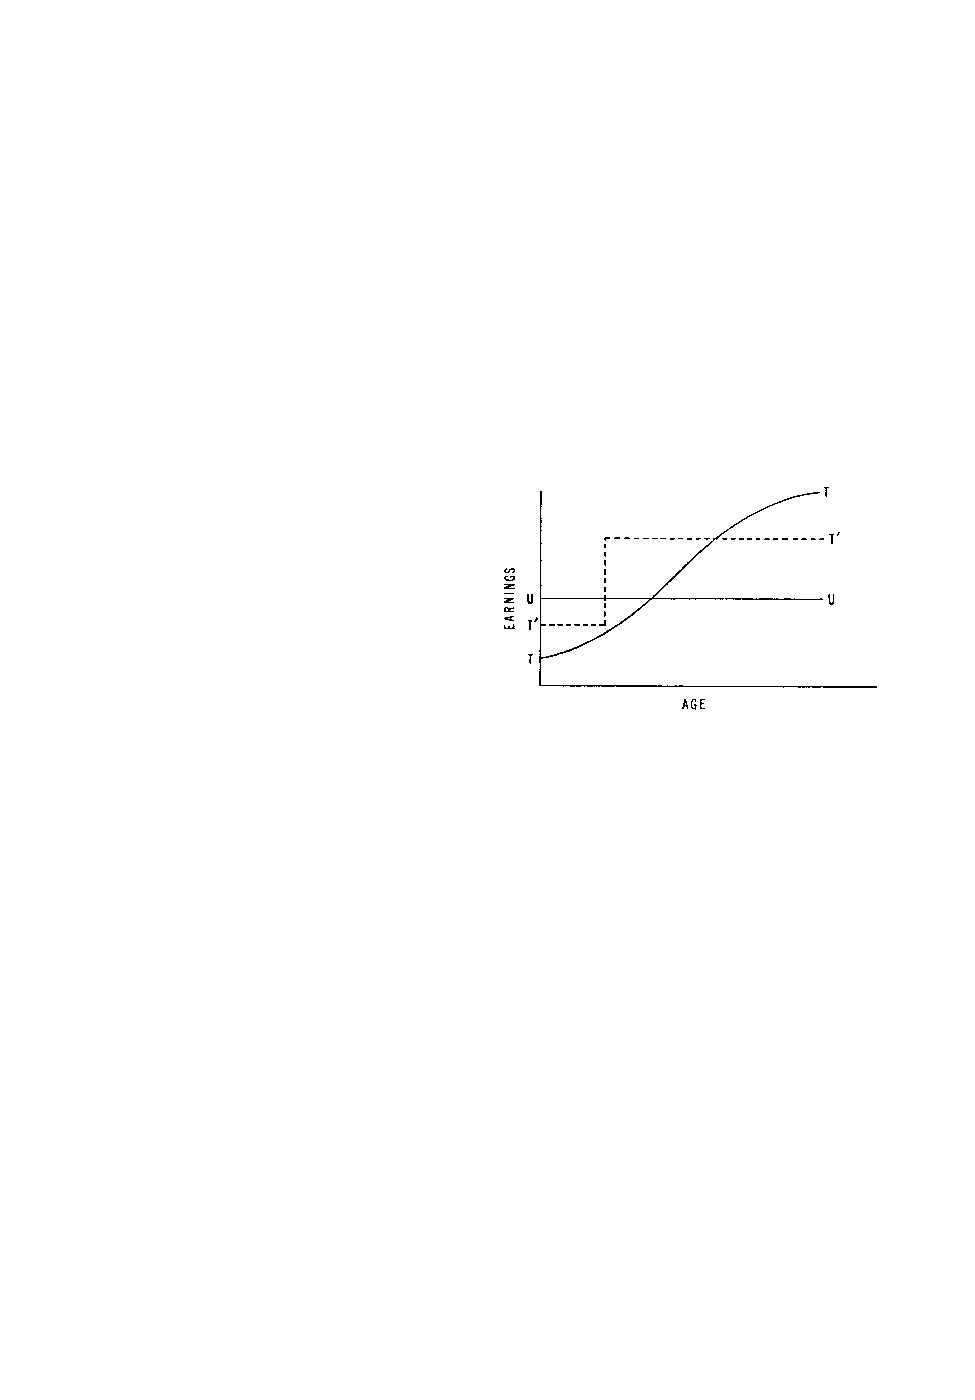
\includegraphics[width=8cm]{fig1.pdf}
        \caption{from Becker, p.15}
        \label{fig1}
      \end{figure}
      UU is the untrained person, TT trained person (first paying for, then collecting rent from training). Difference between UU and TT greater the greater the cost of and return from training. Not only does training make the curve steeper, but also more concave. Extreme case TT'.
    \item Unemployment rates tend to be negatively related to the level of skill
      \begin{itemize}
        \item market demand, $MP$...
      \end{itemize}
    \item Firms in underdeveloped countries appear to be more
      "paternalistic" toward employees than those in developed countries
      \begin{itemize}
        \item investment in activities outside the job are done when an
          increase in productivity is the result
        \item e.g. health, anti-alcoholism
        \item thus, this "paternalistic" behavior results from typical
          behavior outside the firm!
      \end{itemize}
    \item Younger persons change jobs more frequently and receive more
      on-the-job training than older persons
      \begin{itemize}
        \item decisions regarding human capital are NPV decisions
        \item therefore, they are driven by the time-frame of the
          decision (on-the-job training)
      \end{itemize}
    \item The distribution of earnings is positively skewed, especially
      among professional and other skilled workers
    \item Abler persons receive more education and other kinds of
      training than others
      \begin{itemize}
        \item higher $MP$...
      \end{itemize}
    \item The division of labour is limited by the extent of the
      market
      \begin{itemize}
        \item a larger market generates \emph{incentives} for more
          specialization, as higher investments in education are
          rewarded by higher wages
        \item thus, a "larger market" implies more demand for
          specialized skills...
      \end{itemize}
    \item the typical investor in human capital is more impetuous and thus
      more likely to err than is the typical investor in tangible capital
  \end{enumerate}
  % section stylized facts (end)

  \subsubsection{Basic Model} % (fold)
  \label{sec:model}
  \begin{eqnarray}
    MP &=& w
  \end{eqnarray}
  Workers have different unique productivities (wages) in each period.
  \begin{eqnarray}
    MP_{t}&=&w_{t}
  \end{eqnarray}
  Training lowers current receipts (R) and raises current expenditures
  (E). However this trend is reversed for future periods. Therefore: NPV
  consideration.
  \begin{eqnarray}
    \sum_{t=0}^{n-1} \dfrac{R_t}{(1+i)^{t+1}} &=& \sum_{t=0}^{n-1}
    \dfrac{E_t}{(1+i)^{t+1}}
  \end{eqnarray}
  Now we only have training in the first period; Expenditures in first
  period are wages + cost of training (k); afterwards only wage. Receipts
  in all periods is MP.
  \begin{eqnarray}
    MP_0 + \sum_{t=0}^{n-1} \dfrac{MP_t}{(1+i)^{t}} &=& W_0 + k +
    \sum_{t=0}^{n-1} \dfrac{W_t}{(1+i)^{t}} \label{eq4}
  \end{eqnarray}
  We define term $G$
  \begin{eqnarray}
    G&=& \sum_{t=1}^{n-1} \dfrac{MP_t - W_t}{(1+i)^{t}}
  \end{eqnarray}
  Now equation (\ref{eq4}) becomes
  \begin{eqnarray}
    MP_0 + G &=& W_0 + k \label{eq6}
  \end{eqnarray}
  Now we need to include the fact that training takes away time from
  production. ($MP'_0$ what could have been produced, $MP_=$ what was
  actually produced, C is the sum of opportunity cost and the outlays on
  training) Equation (\ref{eq6}) becomes
  \begin{eqnarray}
    MP'_0 + G &=& W_0 + C \label{eq7}
  \end{eqnarray}
  We see that G is the excess of future receipts over future outlays (a
  notion of return on training). Optimality condition: $G=C$ (return
  equals cost)
  % section model (end)

  \subsubsection{General Training} % (fold)
  \label{sub:general_training}
  \textbf{General Training:} This kind of training generally increases
  the $MP$ of the worker. Since the worker can switch jobs, he will
  have to bear the costs of this kind of training.

  Hence, $MP$ and $W$ are raised by the same amount! $MP_t = W_t
  \forall t$ 
  \begin{eqnarray}
    G&=& \sum_{t=1}^{n-1} \dfrac{MP_t - W_t}{(1+i)^{t}}=0
  \end{eqnarray}
  Thus, eq. (\ref{eq7}) becomes 
  \begin{eqnarray}
    MP'_0 &=& W_0 +C \\
    \rightarrow W_0 &=& MP'_0 -C
  \end{eqnarray}
  % subsection General Training (end)
  \subsubsection{Specific Training} % (fold)
  \label{sub:Specific_Training}
  \textbf{Specific Training:} This kind of training only increases the
  $MP$ of the worker for the specific firm.
  Consequently, in this extreme case firms are willing to pay for the
  training, since the investment is offset by increases in profit due
  to higher $MP$ of the workers. On the other hand, workers will not
  be willing to invest, since they have "no gain" from this kind of
  investment. The gain is fully absorbed by the firm!
  % subsubsection Specific Training (end)

  \subsection{(Ben-Porath, 1967) "The Production of Human Capital and the Life Cycle of Earnings"} % (fold)
  \subsubsection{Assumptions}
    
  \subsubsection{Fact sheet} % (fold)
  \begin{enumerate}
    \item People make most of their investments in themselves when they are young, and to a large extend by foregoing current earnings.
    \item The larger the stock of human capital, the larger the earnings per unit of time that the individual could get in the market and therefore the higher the foregone earnings from diverting a unit of time away from the market.
    \item If $\gamma _{1} = \gamma _{2}$ (Cobb-Douglas: Equation (17), p. 360) the more highly educated person is also better equipped for learning, so that his higher opportunity cost is matched by the greater amount of skills that he can acquire per hour.
    \item If $\gamma _{2} > \gamma _{1}$ capital accumulation reduces the cost of producing human capital, and it is possible even in phase (ii) to have a stretch of time over which investment rises.
    \item Three phases will exist:
      \begin{itemize}
        \item Available stock of human capital $K_t$ is not large enough to satisfy demand.
        \item Available stock is enough to supply the services demanded, so that $0<s<1$ and the services of human capital are truly a variable factor.
        \item Stock of capital is too big so that the optimal policy requires more disinvestment than is feasible through deterioration, that is to produce negative quantities of human capital.
      \end{itemize}
    \item \emph{Normal case}: Capital stock does rise over a period, eventually as gross additions become very small and the stock becomes large this must be reversed, and toward end of life, $T$, the stock will decline, if there is any deterioration.
    \item $\dot{I}$ is always negative. Thus the curve of observed earnings exaggerates the rate of increase of earning capacity when the latter increases and understates its decline when it declines.
    \item If depreciation is zero, there is always, except at point $T$, an increase in the three types of earnings ($E_t$ - disposable earnings, $Y_t$ - earning capacity, $\hat{E}$ - observed earnings), and at each point in time their rank by rate of change will be the reverse of their rank by level.
    \item If there is no deterioration ($\delta = 0$) the ever rising curve of observed earnings is always concave from below.
    \item Possibility that optimal decision requires initial assignment of $s=1$, or $100\%$ of the labour force educating themselves.
  \end{enumerate}

  \subsection{(Lazear, 2003) "Firm-Specific Human Capital: A Skill-Weights Approach"} % (fold)
  \subsubsection{Fact sheet} % (fold)
  \begin{enumerate}
    \item The ``skill-weights" view allows skills to be general instead of firm-specific. Instead the relative importance of skills makes them more or less attractive to employers.
    \item $y_i = \lambda_i A+(1-\lambda_i)B$ is the potential earning for a worker with skill set $(A, B)$ at firm $i$.
    \item $\lambda_i$ reflects that firm $i$ may weigh the two skills differently.
    \item $p$ is the probability that the worker is going to stay with the current company in the next period.
    \item The difference between the earnings growth associated with a given amount of experience for those who stay and those who go leads on the \emph{tenure coefficient}. The amount of wage growth the leavers get loads on the experience coefficient.
    \item The worker must chose his investment strategy not knowing whether he will leave the firm or not. $p$ is usually large enough so that he caters to the needs of the first job. When he looses his job he will also loose some income since his skill set will most likely be poorly matched to the new job.
    \item The lower $p$, the less he looses through being let off.
    \item The tenure coefficient should be negatively related to the amount of turnover in the occupation.
    \item Those who leave a firm with unusual weighting patterns suffer larger wage loss for a given $p$.
    \item $Market thickness$ is modeled as allowing more search: Two draws occur, for the second of which the worker can decide whether to switch jobs or not.
    \item In thicker markets a worker looses less on a move despite a more idiosyncratic investment strategy.
    \item Investment increases over time because except for a perfect match between the preferences of the first and second company another round of investment is appropriate.
    \item Shown with data: It is possible to generate tenure coefficients that are nearly the same size as the experience coefficients ($90\%$).
    \item The higher $p$, the large the tenure coefficient.
    \item When $\lambda$ takes extreme values it tends to be far away from $\bar{\lambda}$, which is why the uniform distribution yields lower tenure coefficients than the bimodal.
  \end{enumerate}

  \section{Meeting 4} % (fold)
  \label{prt:Meeting 4}
  \subsection{(Destré et al., 2006) "Learning form experience or learning from others?"} % (fold)
  \label{sec:Destré et al., 2006}
  \setcounter{equation}{0}
  \subsubsection{Introduction} % (fold)
  \label{ssub:Introduction}
  \begin{itemize}
    \item Mincerian earnings function: Linear in education, quadratic in labor market experience.
    \item extended version: includes a quadratic funtion of tenure in the incumbent firm
  \end{itemize}
  Here, the authors have a dataset based in France, of 150,000 wage earners and 16,000
  establishments. They furthermore distinguish informal training by means of learning from own
  experience and learning from others.

  \subsubsection{Informal learning on-the-job from self and others: theory} % (fold)
  \label{ssub:Informal learning on-the-job from self and others: theory}
  \begin{itemize}
    \item workers acquire job-specific training, either formally or informally. Both forms are
      costly, but the difference is that purely informal learning does not take time away from
      others.
    \item informal training often depends on the work contract. workers are "forced" to acquire the
      knowledge of the firm. Thus, workers bear the cost of training, but also reap the rewards.
  \end{itemize}
  Formally, for worker $i$ in firm and job $j$ and time period $t$: Job-specific human capital
  $h_{ijt}$. $H_{ijt}$ is the human capital level of the "teacher" for informal learning. Factor
  $g$ is the depreciation rate of human capital (normally positive). $n$ is the rate of knowledge
  diffusion in the firm.
  \begin{eqnarray}
    h_{ijt}- h_{ij,t-1} &=& gh_{ij,t-1}+ \dfrac{n}{1+n}(H_{ij,t-1} - h_{ij,t-1} ), \forall t \geq
    1
  \end{eqnarray}
  Furthermore, it is shown how job-specific human capital grows with "tenure" (time on the job).
  \setcounter{equation}{2}
  \begin{eqnarray}
    h_{ijt} &=& (1+g)^t h_{ij0} (1+(k^t)\lambda_{ij}) , \mbox{  with  } \lambda_{ij} =
    \dfrac{H_{ij0}}{h_{ij0}} -1 \forall \lambda{ij} \geq 0
  \end{eqnarray}
  $\lambda_{ij}$ denotes the job-specific learning from others' potential, it is independent of
  tenure. Now, the equation is converted in natural logarithms (for econometric estimation)
  \begin{eqnarray}
    \log h_{iht} &=& \log h_{ij0} + gt + \log (1+ \lambda_{ij}(1-k^t))
  \end{eqnarray}
  $\lambda$ can probably be approximated:
  \begin{eqnarray}
    \log h_{iht} &=& \log h_{ij0} + gt + \lambda_{ij}(1-k^t) \mbox{  with  } \lambda_{ij} = \log
    \dfrac{H_{ij0}}{h_{ij0}}
  \end{eqnarray}
  Now, the logarithm of gross earnings is the sum of a linear-in-tenure experience effect and an
  exponential effect of learning from others that converges fast towards the firm's job-specific
  learning potential.

  \subsubsection{The returns to tenure} % (fold)
  \label{ssub:The returns to tenure}
  The marginal returns to tenure ($R$) are defined as:
  \begin{eqnarray*}
    R_{ijt} &=& \dfrac{h_{ijt}- h_{ij,t-1}}{h_{ij,t-1}} \mbox{  } \forall t \geq 1
  \end{eqnarray*}
  "after a few manipulations"
  \begin{eqnarray}
    R_{ijt} &=& g + \dfrac{n}{n+1} \left( \dfrac{\lambda_{ij} k^{t-1}}{1+\lambda_{ij}(1-k^{t-1})} \right)
  \end{eqnarray}
  \begin{itemize}
    \item returns to tenure is from dependent
    \item also depends on teacher/worker knowledge ratio
    \item marginal returns to tenure are shown to be a concave increasing function of the
      job-specific learning potential
    \item there is also a convex decreasing relation of the marginal return to tenure with tenure
    \item increasing the efficiency of learning from others on-the-job will benefit low-tenured
      workers who will learn faster, but it will reduce what remains to be learned from others in
      the future
  \end{itemize}
  \begin{eqnarray*}
    \dfrac{\delta R_{ijt}}{\delta g} & \geq & 1, \mbox{  for  } t \geq 2 \mbox{  and  }
    \lambda_{ij} \geq 0 \mbox{  } (=1 \mbox{  if  } \lambda_{ij}=0)
  \end{eqnarray*}
  Increasing the efficiency of experience initially increases the self-learning effect but this will
  provoke a multiplier effect in subsequent periods by raising the firm's knowledge.
  % subsubsection The returns to tenure (end)

  \subsubsection{Data end econometric specification} % (fold)
  \label{ssub:Data end econometric specification}
  Large French cross section with matched employer-employee data, 1992 INSEE survey on labor cost
  and wage structure. Carried out across all EU countries. Regression analysis... additional
  variables defined in table 1 (p. 926).
  % subsubsection Data end econometric specification (end)

  \subsubsection{Informal learning on-the-job from self and others: results} % (fold)
  \label{ssub:Informal learning on-the-job from self and others: results}
  Summary of the results is given in table 2 (p. 929). Core yelling points:
  \begin{itemize}
    \item on average, it takes 1.93 years for a worker to embody 50\% of what she can learn from
      others in her establishment, and 9.37 years to embody 95\% of this in total
    \item in contrast to the mincerian model, the return on education is slightly lower, this is
      because one can "learn less" in the firm (regarding return on tenure!)
    \item less educated workers typically make up for lower education by more work-based learning
  \end{itemize}
  % subsubsection Informal learning on-the-job from self and others: results (end)

  \subsubsection{firm's knowledge and the returns to tenure} % (fold)
  \label{ssub:firm's knowledge and the returns to tenure}
  In terms of core yelling points: if there is more knowledge in the firm, the worker will have
  (depending on the functional form that is specified in the model) a generally higher return on
  tenure, since he will be able to learn more!
  % subsubsection firm's knowledge and the returns to tenure (end)


  \subsubsection{job heterogeneity} % (fold)
  \label{ssub:job heterogeneity}
  The teacher/woker knowledge ratio is quite different per firm. They then divide jobs in two
  categories, imitation jobs and experience jobs. Jobs that have a low potential to learn from
  others are called experience jobs. When you can learn from others: Imitation job. Majority of jobs
  are imitation jobs, only 15.8\% of jobs are classified as experience jobs. Return on tenure and
  t/w ratio differ for these jobs!  See table 6 (p. 933).
  % subsubsection job heterogeneity (end)

  \subsubsection{dualism at the establishment's level} % (fold)
  \label{ssub:dualism at the establishment's level}
  (Establishment: Employer) ... same conclusions can be drawn ...
  % subsubsection dualism at the establishment's level (end)

  \subsubsection{learning from jobs or learning from firms?} % (fold)
  \label{ssub:learning from jobs or learning from firms?}
  See figure 2 (p. 935), the rate of return to tenure is strongly decreasing for imitation jobs,
  whereas it stays constant for experience jobs! Furthermore, the average marginal rate of return to
  self-learning is considerably higher for experience jobs than for imitation jobs. Workers with
  experience jobs don't learn from others but by themselves. The marginal returns to education are
  lower in imitation jobs, more educated workers have less to learn from others.
  % subsubsection learning from jobs or learning from firms? (end)

  \subsubsection{conclusions} % (fold)
  \label{ssub:conclusions}
  Taken directly from article:\\
  We have suggested a simple model of informal learning on-the-job which combines learning from (own)
  experience and learning from others. This yields a closed-form solution that revises the
  Mincer–Jovanovic’s (1981) treatment of tenure in the human capital earnings function by relating
  earnings to the individual’s job-specific learning potential. We estimated the structural parameters
  of this non-linear model on a large French cross-section with matched employer–employee data. We
  find that workers on average can learn from others 10\% of their own human capital on entering the
  firm, and catch half of their learning potential in just 2 years. Since individuals learn fast from
  their co-workers, the estimated returns to tenure loom larger than predicted by a quadratic, or even
  a quartic-in-tenure, Mincerian function in the first years and decline more sharply (until about 30
  years). Learning by watching accounts for three quarters of the marginal rate of return in the first
  year of tenure, but this share falls rapidly, with an average of 12\%. While education and
  self-learning on-the-job are complementary, education and learning from others on-the-job are
  substitutes. The more education, the less can be learned from others. This forces the private
  marginal return curve to decline with education, an effect which was not captured by current theory.
  Seen from a different perspective, the more educated workers share the social returns of their own
  education with their less qualified co-workers.  The potential for learning from others on the job
  varies across jobs and establishments, and this provides a new distinction between imitation jobs
  and experience jobs. Workers in imitation jobs, who learn most from others, tend to have
  considerably longer tenure than workers in experience jobs. The latter are more mobile and have
  accumulated more market experience. Although workers in experience jobs can learn little from
  others, we find that they learn a lot by themselves. Consequently, we do not find a close
  correspondence between the imitation jobs/experience jobs “dualism” and the primary/secondary jobs
  and firms’ dualism implied by the dual labor market theory. Even though imitation jobs imply far
  less turnover than experience jobs, imitation jobs do not appear to be “better” in terms of
  education levels and wages. We show, however, that predictions of the dual labor market theory which
  cannot be observed at the job’s level under our classification of jobs emerge from the aggregation
  of jobs at the establishment level. Furthermore, we find no evidence of rationing of primary-type
  jobs and establishments. Competition prevails between jobs and firms but jobs differ by their
  learning technology. Firms that make an intensive use of learning from others adhere rather
  naturally to more collective forms of workers’ governance such as reliance to trade unions in
  comparison with those that make an intensive use of self-learning.

  % subsubsection conclusions (end)

  \subsection{(Ertaut, 2000) "Non-formal learning and tacit knowledge in professional work"} % (fold)
  \label{sec:(Ertaut, 2000}

  % section (Ertaut, 2000 (end)
  % part Meeting 4 (end)



  %\bibliographystyle{apacite} 
  %\bibliography{lit}
\end{document}
